\documentclass{article}
\usepackage{listings}
\usepackage{geometry}
\usepackage{amsmath,amsthm,amssymb}
\usepackage{hyperref}
\usepackage{color}
\usepackage{mathtools}
\usepackage{tikz-cd}

% mathbb shortcuts
\newcommand{\Z}{\mathbb{Z}}
\newcommand{\N}{\mathbb{N}}
\newcommand{\Q}{\mathbb{Q}}
\newcommand{\R}{\mathbb{R}}
\newcommand{\C}{\mathbb{C}}
\newcommand{\F}{\mathbb{F}}
\newcommand{\T}{\mathbb{T}}
\newcommand{\HH}{\mathbb{H}}
\newcommand{\RP}{\mathbb{RP}}
\newcommand{\PP}{\mathbb{P}}
\newcommand{\A}{\mathbb{A}}
\newcommand{\E}{\mathbb{E}}

% mathfrak shortcuts
\newcommand{\fI}{\mathfrak{I}}
\newcommand{\fA}{\mathfrak{A}}
\newcommand{\fG}{\mathfrak{G}}

% mathcal shortcuts
\newcommand{\cA}{\mathcal{A}}
\newcommand{\cU}{\mathcal{U}}
\newcommand{\cR}{\mathcal{R}}
\newcommand{\cP}{\mathcal{P}}
\newcommand{\cB}{\mathcal{B}}
\newcommand{\cC}{\mathcal{C}}
\newcommand{\cF}{\mathcal{F}}
\newcommand{\cS}{\mathcal{S}}

\newcommand{\Aut}{\textrm{Aut}}
\newcommand{\degg}{\textrm{deg}}
\newcommand{\Hom}{\textrm{Hom}}
\newcommand{\conj}{\textrm{conj}}
\newcommand{\Gal}{\textrm{Gal}}
\newcommand{\disc}{\textrm{disc}}
\newcommand{\supp}{\textrm{supp}}
\newcommand{\Jac}{\textrm{Jac}}
\newcommand{\Der}{\textrm{Der}}
\newcommand{\Spec}{\textsf{Spec}\,}
\newcommand{\im}{\textrm{im}\,}

% mathsf shortcuts
\newcommand{\Cell}{\textsf{Cell}}

\newcommand{\clr}{\color{red}}

\newtheorem{lemma}{Lemma}
\newtheorem{definition}{Definition}
\theoremstyle{definition}


\begin{document}

\begin{center}
	\large \textbf{GRST Notes: Research Ideas (January 25, 2017)} \\
\end{center}

This week, Sam talked about some ideas he had about possible directions for research. 

\section{Random Sheaves 1}
An interesting concept to consider is the notion of a random sheaf, and how to properly define one. We will discuss two methods to do this assuming we have some initial data: a top-down method in which the initial data is defined on maximal cells, and a bottom-up method in which the initial data is defined on a graph.\\

We begin with Sam's algorithm to construct a random sheaf from the top down; we'll continue with the other method in the third section. The aim is to define a sheaf on a fixed cell complex $X$. Suppose that the stalk over each cell is predetermined (we choose a vector space for each cell), and that all maps into maximal cells (cells that are not the face of any other cell in $X$) are predetermined. For example, if we begin with the following cell complex, all of the arrows in red must be predetermined. Note that although the edge on the side is not a cell of maximum dimension, it is not the face of any other cell.

\begin{figure}[!htbp]
\centering
	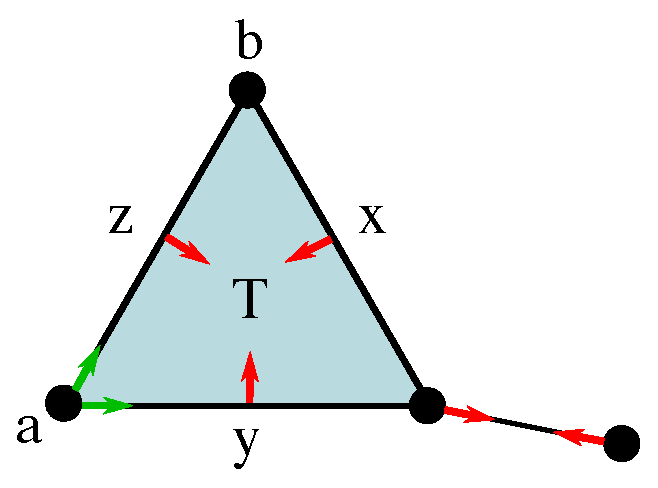
\includegraphics[width=0.3\textwidth]{images/cellcomp.eps}
\end{figure}

Given this initial data, the idea is to define all the other maps in the sheaf such that all of the commutativity relations are preserved. This is done by taking categorical limits. Suppose we want to define the green maps out of $a$; it turns out that we can define all maps coming out of a single cell all at once. 

\begin{definition} Suppose $(P, \leq)$ is a pre-order. The \textbf{open star} of a point $x \in P$ is defined to be the set $U_x = \{y \in P \, | \, x \leq y\}$.
\end{definition}

The open star is simply the set of higher-dimensional cells of which the cell $x$ is a face. Viewing the cell complex $X$ as a poset, we take the open star of the cell $a$, along with all maps connecting these points, shown in the following diagram.

\[
\begin{tikzcd}
	& T & \\
	z \arrow[red]{ur} &  & y \arrow[red]{ul} \\
	& a \arrow[green]{ul} \arrow[green]{ur} & 
\end{tikzcd}
\]

Next, we remove $a$ and all maps out of $a$ from the open star (which we call the reduced open star {\clr is this bad terminology?}), and we take the limit of the reduced open star. This gives us a vector space $L$, and two maps $p_1 : L \rightarrow z$ and $p_2: L \rightarrow y$. We then choose a random map $\alpha: a \rightarrow L$, and the green arrows are then defined by composition. Explicitly, we have $\phi_1 = p_1 \circ \alpha$ and $\phi_2 = p_2 \circ \alpha$.  This scenario can be seen in the following diagram. 

\[
\begin{tikzcd}
	& T & \\
	z \arrow[red]{ur} &  & y \arrow[red]{ul} \\
	& L \arrow[swap,"p_1"]{ul} \arrow["p_2"]{ur} & \\
	& a \arrow{u}{\alpha} \arrow[green,bend left]{uul}{\phi_1} \arrow[swap, green, bend right,"\phi_2"]{uur} &
\end{tikzcd}	
\]

Repeating this procedure for all other $0$ cells, we obtain a consistent set of maps between cells of $X$, and we have thus defined a sheaf on $X$.\\

This was a fairly simple example to complete, but the algorithm is similar for cell complexes with higher dimensional cells. The main difference is that we must perform this algorithm dimension by dimension starting from the highest dimension in the cell complex, and working our way down. Specifically, if the highest dimensional cell is of dimension $n$, then all maps out of $(n-1)$ cells are pre-determined, so the first step is to determine the maps out of $(n-2)$-cells. The reduced open star only includes higher dimensional cells, so we can exactly follow the procedure described above. After all maps out of $(n-2)$ cells are defined, we move on to $(n-3)$ cells, and continue this iteratively until all maps are defined. \\


\section{Moduli Spaces of Sheaves 1}
It would be interesting to understand all possible sheaves constructed in this manner, given that we start with a cell complex $X$, the vector space over all cells, and maps into the maximal cells. There are two different viewpoints that we can take with this: an iterative viewpoint mimicing the iterative process to build the random sheaf, and a consolidated viewpoint which looks at entire procedure all at once.\\

Consider the construction of the sheaf in the previous section. For concreteness, suppose that the vector spaces over the cells $z$ and $a$ are $z =k^p$ and $a = k^q$, where $k$ is a field. Any map $\phi_1 : k^m \rightarrow k^n$ can be represented as a matrix $(x_{i,j})_{1\leq i \leq p, 1 \leq j \leq q}$ of $pq$ variables, so we can think of any such matrix as being a point in $k^{nm}$. We obtain one matrix for each map we aim to define. The space of all matrices for maps coming out of $0$-cells is $k^{N_0}$, where $N_0$ is the sum of the number of variables for each of these matrices. \\

However, not all choices of matrices will result in a sheaf. Enforcing the commutativity of the diagram will give us a collection of polynomial equations where the variables are elements of these matrices; we denote this collection of equations $\cP_0$. Therefore, a consistent set of matrices that satisfies all the sheaf conditions is a point in $k^{N_0}$ that satisfies all polynomial equations in $\cP_0$. In other words, it is a point on the variety $S_0 = V(\cP_0)$ in $k^{N_0}$, as shown in the figure below.\\

\begin{figure}[!htbp]
\centering
	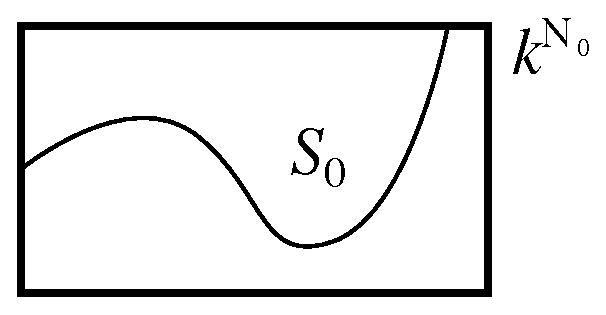
\includegraphics[width=0.3\textwidth]{images/variety1.eps}
\end{figure}

In the case of the cell complex above, $S_0$ defines the space of all possible sheaves, since the construction is complete after defining maps out of the $0$-cells. However, suppose that the maximum dimension in the cell complex is $n$. By the initial data, the maps out of $(n-1)$ cells are predefined, so the first step is to define the maps out of $(n-2)$ cells. By the argument above, the space of all possible maps out of $(n-2)$ cell is $k^{N_{n-2}}$, where $N_{n-2}$ is the number of variables for each of these matrices. We will get a collection of polynomials, $\cP_{n-2}$, that these must satisfy, and the resulting variety is $S_{n-2} = V(\cP_{n-2})$. After choosing a point in this variety, we continue this procedure until we reach the variety $\cS_0$. Then, any point in $S_0$ will result in a sheaf. However, the important point to note is that each variety $S_i$ is dependent on the choice of point in the previous variety $S_{i+1}$. 

\begin{figure}[!htbp]
\centering
	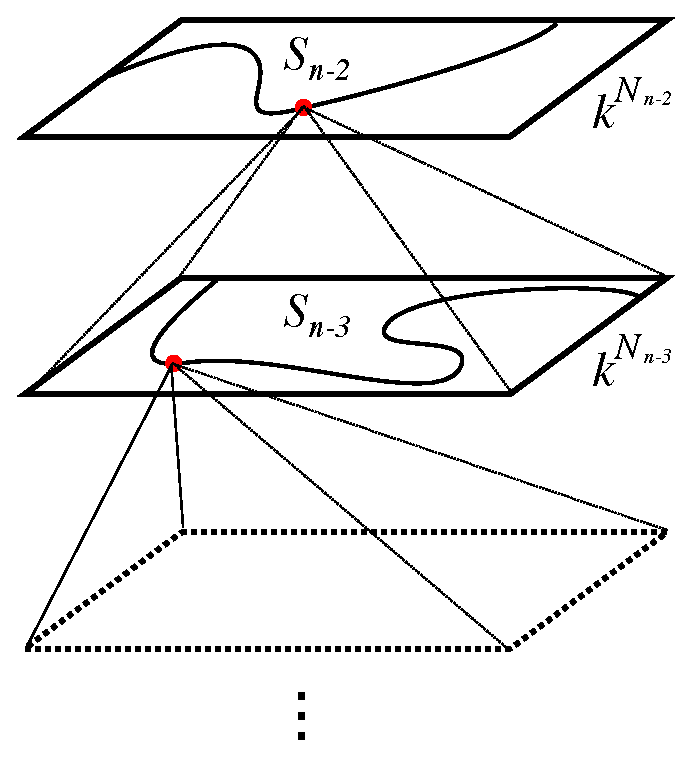
\includegraphics[width=0.3\textwidth]{images/variety2.eps}
\end{figure}

{\clr This is my understanding of this moduli space stuff but I'm not 100 percent sure.} An interesting question to consider is what is the set of all possible sheaves given our initial data? Moreover, what would the moduli space of all possible sheaves look like if we consider sheaves with the same cohomology to be equivalent?

\section{Moduli Spaces of Sheaves 2 and Approximate Sheaves}
Next, we will consider the consolidated approach. Instead of looking at this procedure iteratively, we can look at all of the matrices for all of the unknown maps at once. The set of all such matrices would be in $k^N$, and we would get a large collection of polynomials $\cP$, which would form a variety $S = V(\cP)$. We can ask similar questions here. What would the variety $S$ look like? What would the moduli space of sheaves look like?\\

The idea is that of an approximate sheaf {\clr is this what we want to call it?}. {\clr Sam had two possible ways to get approximate sheaves but I don't quite remember what they were.} When we obtain sheaves in real life, it is highly unlikely that all of the maps will commute properly, but it may be ``close'' to being a sheaf. Is there a way to put a metric on the space $k^N$ and ask what is the closest sheaf to the approximate sheaf?

\begin{figure}[!htbp]
\centering
	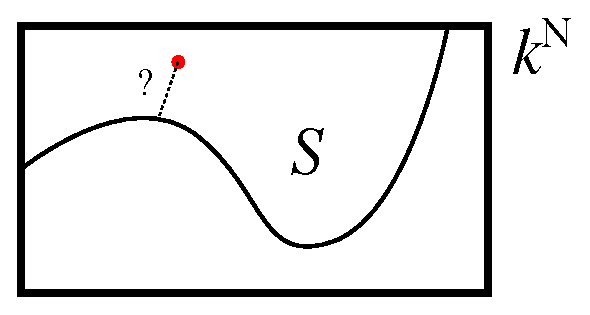
\includegraphics[width=0.3\textwidth]{images/variety3.eps}
\end{figure}


\section{Random Sheaves 2}
While discussing the above top-down method for building a random sheaf, Jakob suggested an alternative bottom-up method for building random sheaves. This idea extends the concept of building a clique complex from a graph. Here, we begin with a sheaf on a graph $X_1$. This implies the stalks over all cells in the graph are chosen, and a consistent set of maps from $0$ cells into $1$ cells is also chosen. For this post, we will use the following graph as an example.\\

\begin{figure}[!htbp]
\centering
	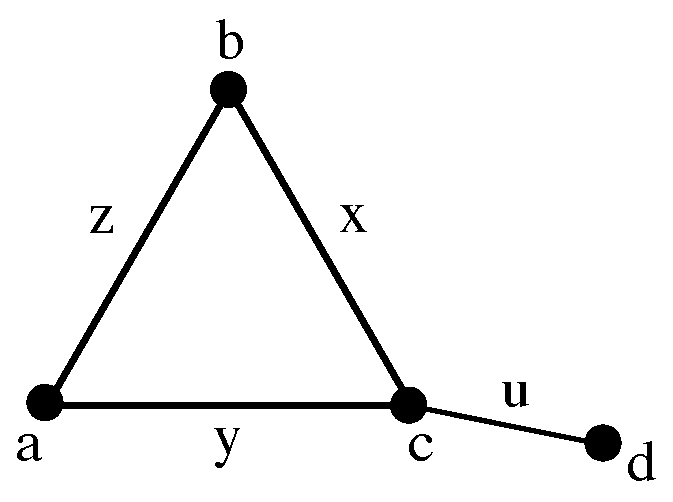
\includegraphics[width=0.3\textwidth]{images/graph.eps}
\end{figure}

Now, we consider the clique complex $X$ of this graph and we denote its $n$-skeleton by $X_n$. We will iteratively define the stalks and maps in the higher dimensional cells beginning with $X_2$. The $2$-skeleton of the clique complex of the above graph is shown in the following figure.

\begin{figure}[!htbp]
\centering
	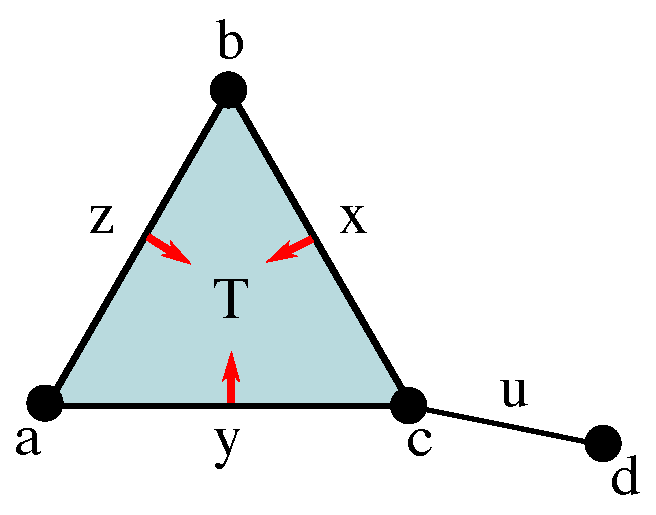
\includegraphics[width=0.3\textwidth]{images/graph2.eps}
\end{figure}

During this step, we must define the stalks on all $2$ cells and also all maps into $2$-cells. In our example, we must define the stalks over $T$ and define the maps represented by the red arrows. This is done in a way that is dual to the method in the first section. 

\begin{definition} Suppose $(P, \leq)$ is a pre-order. The \textbf{closure} of a point $x \in P$ is defined to be the set $V_x = \{y \in P \, | \, y \leq x\}$.
\end{definition}

Here, we are simply taking all lower dimensional cells that are faces of the given cell $x$. Now, we take the closure of the cell $T$, along with all maps between the points in the closure. We remove $T$ along with all maps into $T$ and denote this the \textbf{reduced closure} of $x$ ({\clr again, I'm not sure if this terminology is okay}). We define the stalk over $T$ to be the colimit of reduced closure of $T$, and the maps into $T$ to be the associated maps into the limit.

\[
\begin{tikzcd}
	& T & \\
	x \arrow[red	]{ur} & y \arrow[red]{u} & z \arrow[red]{ul} \\
	a \arrow{ur} \arrow{urr} & b \arrow{ur} \arrow{ul} & c \arrow{ul} \arrow{ull}
\end{tikzcd}	
\]

In the case of this example, we are done. However, if there were more $2$-cells, we would simply repeat this procedure until we have a sheaf on $X_2$. Then, we continue this process for higher dimensional cells until we have a sheaf on $X$. \\

Note that using this bottom-up method, the sheaf on the graph was the only data we needed to predetermine. All other stalks and maps are well-defined using this colimit procedure. Thus, each sheaf on a graph will result in a unique sheaf on its clique complex with this algorithm. In contrast, in the top-down method, we needed to choose a random map into each limit when defining maps into the lower dimensional cells, so we get a space of possible sheaves, as described in sections 2 and 3. \\

One interesting aspect of this bottom-up approach is that we can build a random sheaf by defining a random graph. It would be interesting to study asymptotic properties of random sheaves built in this manner, since this is similar to how random graph theory was extended to random clique complexes in the work of Kahle ({\clr cite something}). 

\end{document}